\documentclass[10pt]{beamer}

\usepackage{ctex}
\setmainfont{Times New Roman}
\setsansfont{Arial}
\setmonofont{Courier New}
\usepackage{booktabs}
\usepackage{amsmath,amssymb,amsfonts}
\usepackage{graphicx}
\usepackage{subfig}
\usepackage{tikz}
\usepackage{caption}
\setbeamertemplate{caption}[numbered]
\setbeamersize{text margin left=1cm, text margin right=1cm}

% 使用biblatex管理参考文献
\usepackage[backend=biber,style=authoryear]{biblatex}
\addbibresource{citation/references.bib}

% 添加主题
\usepackage{style/ahutheme}

% 设置右下角的logo,注释可以取消
\logo{
\includegraphics[height=1cm]{assets/logo2.png}}

% 标题信息
\title{AHU Slide模板示例}
\subtitle{基于beamer的\LaTeX{} ppt模板}
\author{Yaan \and Laan}
\institute{Anhui University}
\date{\today}

% 在每个section之前插入目录页
% \AtBeginSection[]
% {
%   \begin{frame}
%     \frametitle{\insertsectionhead}
%     \tableofcontents[
%                  sectionstyle=show/shaded, 
%                  subsectionstyle=show/show/hide]
%   \end{frame}
% }

% 分点过多的时候可以用这个
\AtBeginSection[]
{
  \begin{frame}
    \frametitle{\insertsectionhead}
    \begin{columns}[onlytextwidth]
    \begin{column}{0.5\textwidth}
    \tableofcontents[
                 sectionstyle=show/shaded, 
                 subsectionstyle=show/show/hide,
                 sections={1-4}]
    \end{column}
    \begin{column}{0.5\textwidth}
    \tableofcontents[
                 sectionstyle=show/shaded, 
                 subsectionstyle=show/show/hide,
                 sections={5-100}]
    \end{column}
    \end{columns}
  \end{frame}
}

\begin{document}


% 标题页
\begingroup
\setbeamertemplate{headline}{}
\begin{frame}
\titlepage
\end{frame}
\endgroup
% 目录页
\begin{frame}
\setbeamertemplate{headline}{}
\frametitle{目录}
\tableofcontents
\end{frame}


% 目录页(分点过多的时候可以用这个)
% \begin{frame}
% \frametitle{目录}
% \begin{columns}[onlytextwidth]
% \begin{column}{0.5\textwidth}
% \tableofcontents[sections={1-3}]
% \end{column}
% \begin{column}{0.5\textwidth}
% \tableofcontents[sections={4-100}]%数字大没关系
% \end{column}
% \end{columns}
% \end{frame}



% 内容示例
\section{介绍}
\begin{frame}
\frametitle{介绍}
这是使用ahutheme模板创建的演示文稿示例。

\begin{itemize}
  \item 这是一个蓝白主题的演示文稿模板
  \item 使用现代化的设计风格
  \item 支持中文排版
  \item 易于定制和扩展
\end{itemize}
\end{frame}
\section{功能展示}
\subsection{块环境}
\begin{frame}
\frametitle{功能展示}
\framesubtitle{块环境示例}

\begin{block}{普通块}
这是一个普通块环境的示例。
\end{block}

\begin{alertblock}{警告块}
这是一个警告块环境的示例。
\end{alertblock}

\begin{exampleblock}{示例块}
这是一个示例块环境的示例。
\end{exampleblock}
\end{frame}

\section{数学公式}
\begin{frame}
\frametitle{数学公式}

\begin{block}{数学公式示例}
这是一个数学公式示例:
\[ E = mc^2 \]

还有行内公式示例:$\sum_{i=1}^{n} i = \frac{n(n+1)}{2}$

多行公式示例:
\begin{align}
  f(x) &= x^2 + 2x + 1 \\
  g(x) &= \int_0^x f(t) dt
\end{align}

\end{block}

\end{frame}

\section{列表环境}
\begin{frame}
\frametitle{列表环境}
\begin{enumerate}
  \item 这是一个有序列表的第一项
  \item 这是第二项
  \begin{enumerate}
    \item 这是子列表的第一项
    \item 这是子列表的第二项
    \begin{enumerate}
      \item 这是子子列表的第一项
      \item 这是子子列表的第二项
    \end{enumerate}
  \end{enumerate}
  \item 这是最后一项
\end{enumerate}

\begin{itemize}
  \item 这是一个有序列表的第一项
  \item 这是第二项
  \begin{itemize}
    \item 这是子列表的第一项
    \item 这是子列表的第二项
    \begin{itemize}
      \item 这是子子列表的第一项
      \item 这是子子列表的第二项
    \end{itemize}
  \end{itemize}
  \item 这是最后一项
\end{itemize}

\end{frame}

% 两列环境示例
\section{多列布局}
\begin{frame}
\frametitle{两列环境示例}
\begin{columns}
\column[t]{0.5\textwidth}
在这个示例中,我们将展示如何使用两列环境来并排显示内容。这种方法在需要对比不同信息或并排显示文本和图像时非常有用。

例如,我们可以在这边列出一些优点:
\begin{itemize}
  \item 节省空间
  \item 便于对比
  \item 增强可读性
\end{itemize}

\column[t]{0.5\textwidth}
同时在另一边列出一些缺点:
\begin{itemize}
  \item 可能显得拥挤
  \item 需要仔细平衡内容
  \item 在小屏幕上可能显示不佳
\end{itemize}

也可以放置图像或者公式等内容。
\end{columns}
\end{frame}

% 包含图片、表格和tikz绘图的多列示例
\begin{frame}
\frametitle{多列环境:图片、表格和TikZ绘图示例}
\begin{columns}[T]
\column{0.33\textwidth}
\centering
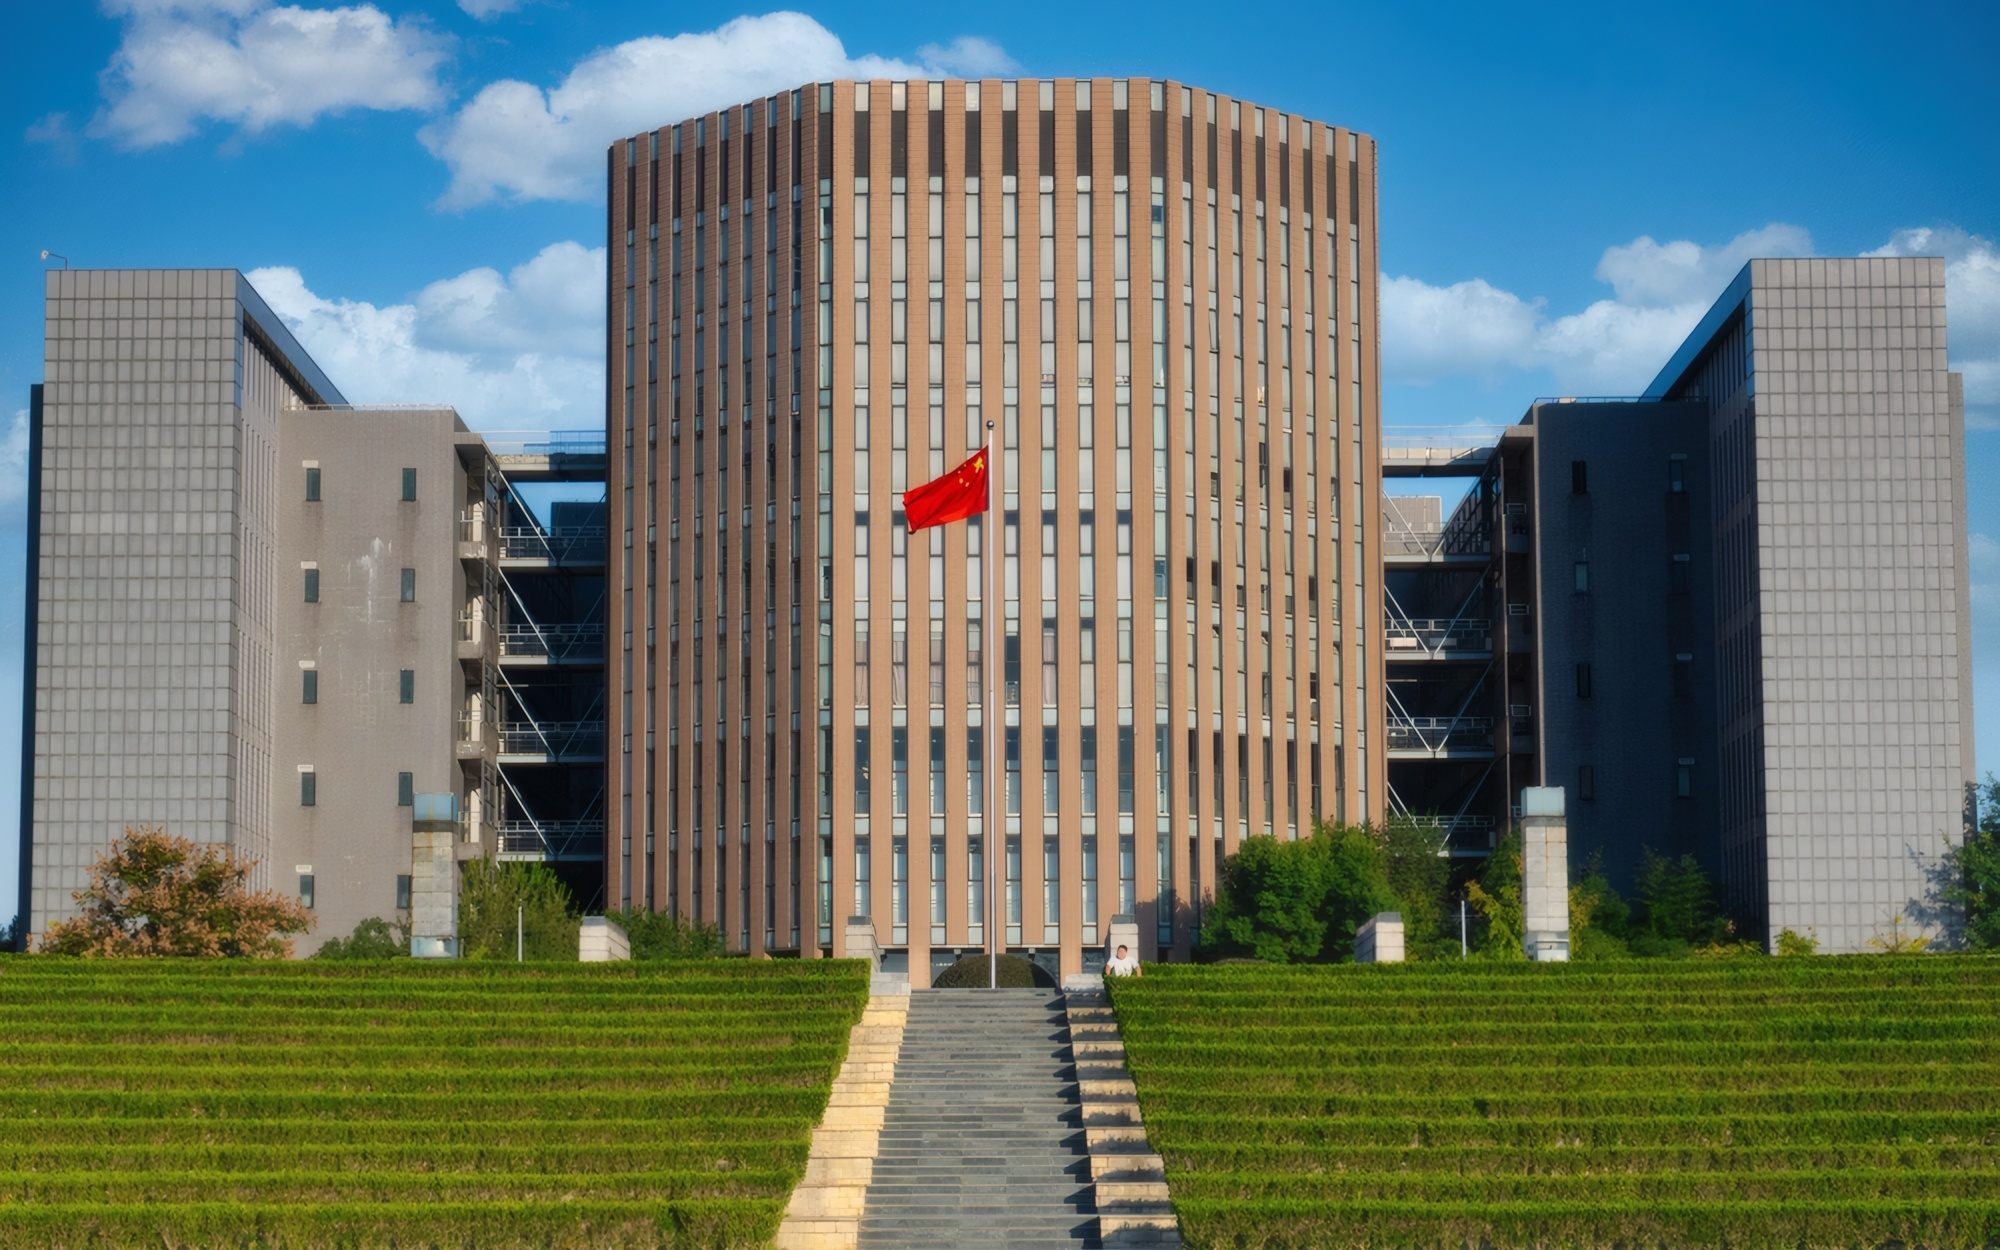
\includegraphics[width=0.7\linewidth]{src/example_ahu.jpg}

\vspace{1em}

\parbox[t]{\linewidth}{
\raggedright
示例图片说明文字\\
这是对图片内容的简要描述
}

\column{0.33\textwidth}
\centering
\begin{tabular}{|c|c|}
\hline
A & B \\
\hline
1 & 2 \\
3 & 4 \\
\hline
\end{tabular}

\vspace{1em}

\parbox[t]{\linewidth}{
\raggedright
示例表格说明文字\\
这是对表格内容的简要描述
}

\column{0.33\textwidth}
\centering
\begin{tikzpicture}
\draw[thick] (0,0) rectangle (1.5,1);
\draw (0.75,0.5) node {示例};
\end{tikzpicture}

\vspace{1em}

\parbox[t]{\linewidth}{
\raggedright
TikZ绘图说明文字\\
这是对绘图内容的简要描述
}
\end{columns}
\end{frame}

\section{图表展示}
% 子图展示示例
\begin{frame}
\frametitle{子图展示示例}
\begin{figure}
\centering
\subfloat[子图A]{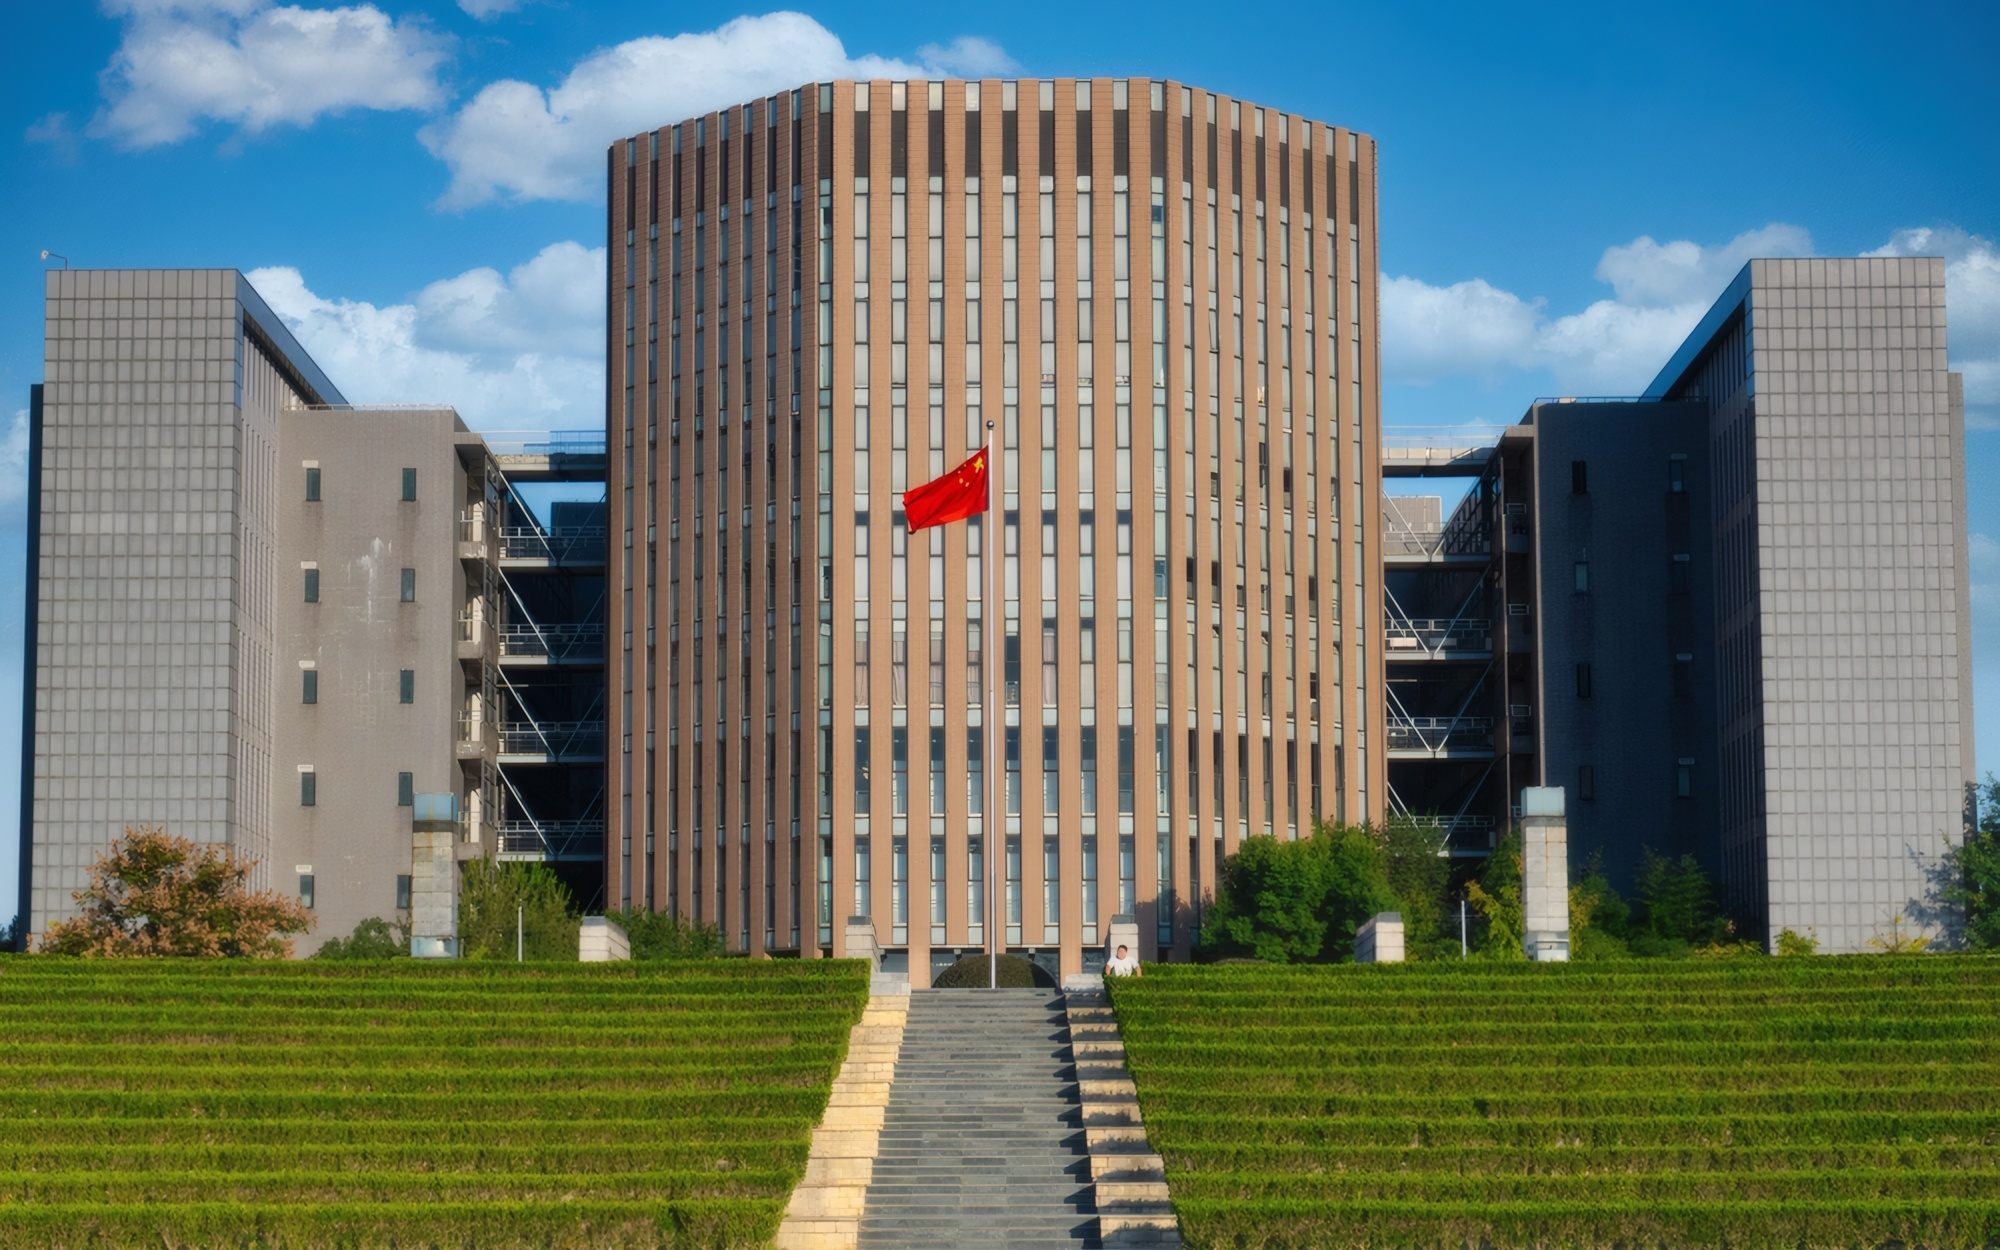
\includegraphics[width=0.45\linewidth]{src/example_ahu.jpg}\label{fig:subfig-a}}
\hfill
\subfloat[子图B]{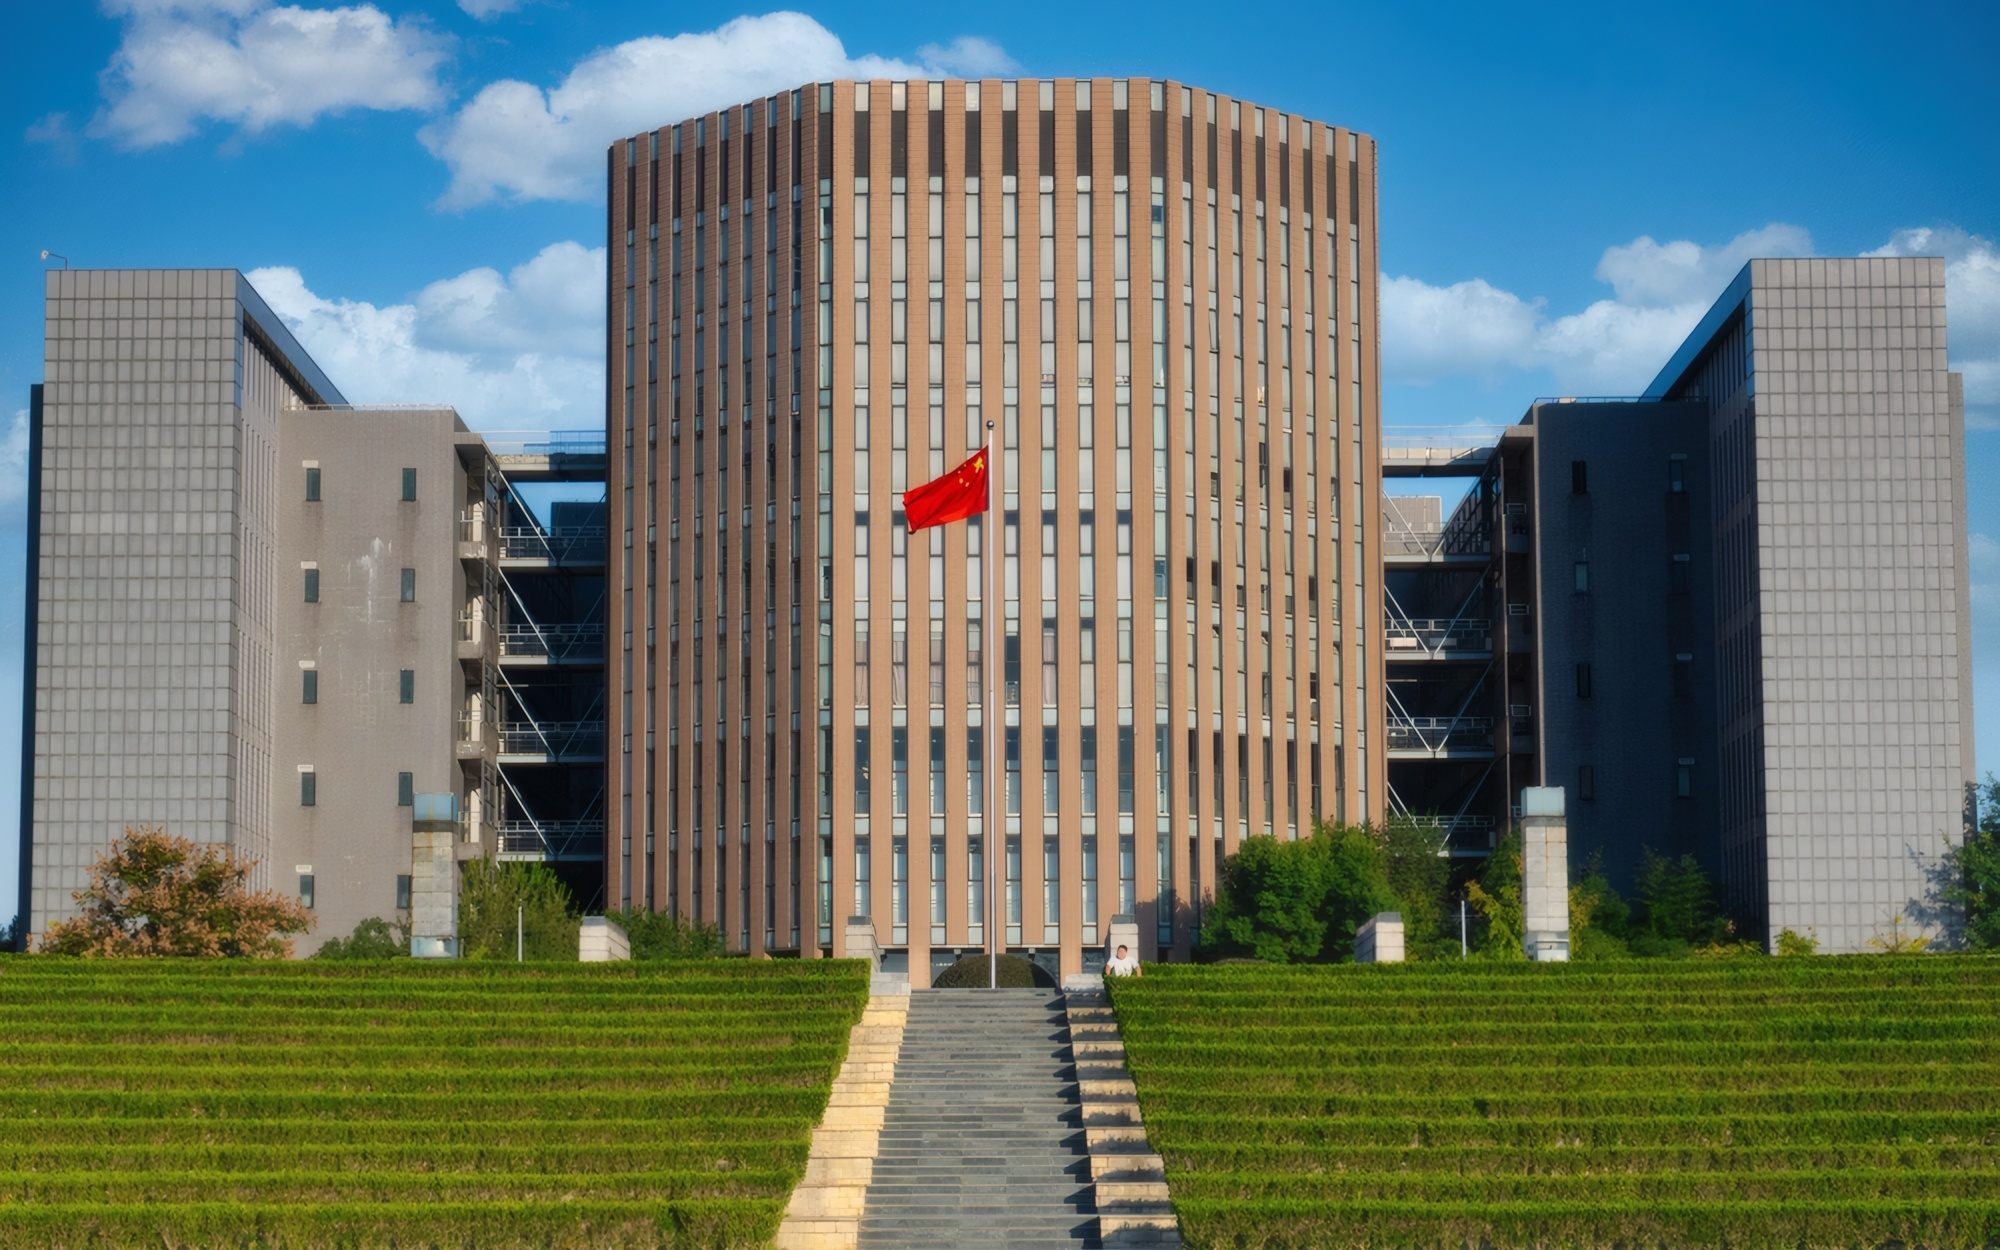
\includegraphics[width=0.45\linewidth]{src/example_ahu.jpg}\label{fig:subfig-b}}
\caption{两个并排的子图示例}
\label{fig:subfigures}
\end{figure}
这是对子图内容的简要描述。
\end{frame}

% 表格展示示例
\begin{frame}
\frametitle{表格展示示例}

\begin{table}[H]
\caption{\textbf{Example 4}}
\centering
\begin{tabular}{cccc}
\toprule
&\multicolumn{2}{c}{Resultsummary}& \\
Item1&Item2&Item3&Item4 \\
\midrule 
Data1&Data2&Data3&Data4 \\
\midrule
Data5&Data6&Data7&Data8 \\
\bottomrule
\end{tabular}
\end{table}


这是对表格内容的简要描述。
\end{frame}

% TikZ绘图示例
\begin{frame}
\frametitle{TikZ绘图示例}
\begin{figure}
\centering
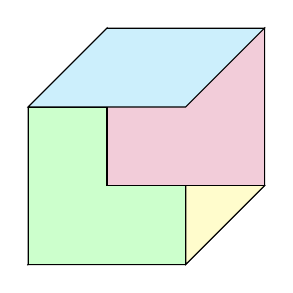
\begin{tikzpicture}[x={(1cm,0cm)}, y={(0.5cm,0.5cm)}, z={(0cm,1cm)}]
  % 绘制立方体
  \draw[fill=blue!20] (0,0,0) -- (2,0,0) -- (2,2,0) -- (0,2,0) -- cycle;
  \draw[fill=red!20] (0,0,0) -- (0,0,2) -- (0,2,2) -- (0,2,0) -- cycle;
  \draw[fill=green!20] (0,0,0) -- (2,0,0) -- (2,0,2) -- (0,0,2) -- cycle;
  \draw[fill=yellow!20] (2,0,0) -- (2,2,0) -- (2,2,2) -- (2,0,2) -- cycle;
  \draw[fill=purple!20] (0,2,0) -- (2,2,0) -- (2,2,2) -- (0,2,2) -- cycle;
  \draw[fill=cyan!20] (0,0,2) -- (2,0,2) -- (2,2,2) -- (0,2,2) -- cycle;
\end{tikzpicture}
\caption{TikZ绘制的示例图形}
\end{figure}
这是对TikZ绘图的简要描述。
\end{frame}
% 参考文献示例
\section{参考文献}
\begin{frame}
\frametitle{参考文献示例}
在文档中引用文献是非常重要的,例如:
\begin{itemize}
  \item Knuth 在其关于文学化编程的文章中提出了相关概念~\cite{knuth1984}
  \item LaTeX 是由 Leslie Lamport 开发的排版系统~\cite{lamport1994}
  \item Till Tantau 开发了 Beamer 类用于制作演示文稿~\cite{tantau2004}
  \item 《The LaTeX Companion》是使用 LaTeX 的重要参考书~\cite{mittelbach2004}
  \item 提出了 Adam 优化算法\cite{kingma2017adammethodstochasticoptimization} 
\end{itemize}
\end{frame}

% 参考文献
\begin{frame}[allowframebreaks]
\frametitle{参考文献}
\printbibliography[heading=bibliography,title=参考文献]
\end{frame}


\begin{frame}
\frametitle{致谢}
\begin{center}
{\Huge THANK YOU !!}\\[1em]
{\Large 月亮想着我的心事,一只猫吃了我的奶酪}
\end{center}
\end{frame}


\end{document}